\documentclass[14pt, oneside]{altsu-report}

\worktype{ОТЧЁТ ПО ТЕХНОЛОГИЧЕСКОЙ (ПРОЕКТНО-ТЕХНОЛОГИЧЕСКОЙ)
ПРАКТИКЕ НА ТЕМУ:}
\title{Разработка игры "Snake" на Unity2D}
\author{Е.\,Д.~Яковенко}
\groupnumber{5.205-2}
\GradebookNumber{1337}
\supervisor{И.\,А.~Шмаков}
\supervisordegree{ст. преп. каф. ВТ и Э}
\ministry{Министерство науки и высшего образования}
\country{Российской Федерации}
\fulluniversityname{ФГБОУ ВО Алтайский государственный университет}
\institute{Институт цифровых технологий, электроники и физики}
\department{Кафедра вычислительной техники и электроники}
\departmentchief{В.\,В.~Пашнев}
\departmentchiefdegree{к.ф.-м.н., доцент}
\shortdepartment{ВТиЭ}
\abstractRU{Объём текста не менее 500 символов! Пока счётчики выставляются в ручную, при необходимости правьте cls-файл.}
\abstractEN{Большой текст на английском!}
\keysRU{компьютерное моделирование, cистема управления версиями}
\keysEN{computer simulation, distributed version control}
\countWorkPage{22}
\countWorkImg{6}
\countWorkLit{5}
\countWorkTab{6}

\date{\the\year}

% Подключение файлов с библиотекой.
\addbibresource{graduate-students.bib}

% Пакет для отладки отступов.
%\usepackage{showframe}

\begin{document}
\maketitle

\setcounter{page}{2}
\makeabstract
\tableofcontents

\chapter*{Введение}
\phantomsection\addcontentsline{toc}{chapter}{ВВЕДЕНИЕ}

\textbf{Актуальность}
\begin{itemize}
\item {Популяризация программирования: Создание игры "Snake" на Unity2D может привлечь новичков к изучению программирования благодаря ее простоте и понятности. Это может быть хорошим стартом для тех, кто только начинает свой путь в мире разработки приложений.}

\item {Обучение и практика: Разработка игры "Snake" на Unity2D может стать отличным учебным проектом для тех, кто хочет попрактиковаться в программировании и улучшить свои навыки разработки игр. Путем создания такого простого, но популярного приложения, можно получить ценный опыт и знания.}

\item {Овладение навыками создания GUI: Разработка игры "Snake" позволит разработчику улучшить навыки создания графического интерфейса (GUI) и работу с анимациями. Это важные навыки для любого программиста, работающего в области разработки приложений.}

\item {Создание функционального приложения: Даже несмотря на свою простоту, игра "Snake" остается популярной и знакомой многим пользователям. Разработка этой игры поможет создать функциональное и привлекательное приложение, которое может привлечь широкую аудиторию.}

\item {Доступность инструментов: Unity2D - это мощный инструмент для разработки игр, который обладает удобным интерфейсом и обширными возможностями. Разработка игры "Snake" на Unity2D может быть отличным способом использовать доступные инструменты для создания нового продукта.}

\end{itemize}

\textbf{Цель:} Разработать функциональную и интерактивную игру «Snake» на
игровом движке Unity, используя при этом:
\begin{itemize}
\item{знания и навыки работы на Unity и программирования на языке C\#.}
\item{методы разработки графического интерфейса пользователя.}
\item{алгоритмы игровой логики.}
\end{itemize}
\textbf{Задачи:}
\begin{itemize}
    \item создать удобный и интуитивно понятный интерфейс для игры
    \item изучить различные варианты реализации игры «Snake»
    \item разработать редактор карт
    \item реализовать несколько режимов игры
    \item реализовать алгоритмы игрового процесса, включая:
    \begin{itemize}
        \item движение змейки и его увеличение
        \item генерация препятствии и их размещение
        \item генерация бомб
        \item генерация еды
        \item счёт очков
    \end{itemize}
\end{itemize}

\textbf{Практическая значимость:}

\begin{itemize}
    \item Развитие навыков: работа над проектом позволит развить навыки программирования, проектирования интерфейсов, тестирования и отладки;
    \item создание готового продукта: результатом работы станет функциональная игра, которую можно использовать для развлечения или в учебных целях;
    \item  возможность применения: полученные навыки могут быть применены для разработки других игр или программных решений.
\end{itemize}



% Подключение первой главы (теория):
\chapter{\label{ch:ch01}ОБЗОР ПРОГРАНЫХ СРЕДСТВ ДЛЯ РЕАЛИЗАЦИИ ИГРЫ <<SNAKE>>} % Нужно сделать главу в содержании заглавными буквами

\section{\label{sec:ch01/sec01}Общие сведения об игре "Snake"}

История игры «Змейка» началась за несколько лет до появления первых мобильных телефонов. В 1977 году компания Gremlin Industries выпустила игровой автомат Hustle, рассчитанный на одного или двух игроков, в которой нужно было управлять «змейками», направляя их на бессистемно появляющиеся цели. Для победы нужно было заполучить больше очков, чем у оппонента, преграждая по ходу игры ему путь к новым целям (в случае многопользовательской игры), или просто побить установленный на игровом автомате рекорд. В 1984 году Gremlin Industries была вынуждена закрыться, но игра Hustle начала набирать обороты: сначала появился порт для компьютеров TRS-80, затем для Commodore PET и Apple II.

Оригинальная «Змейка» (Snake) от Nokia появилась в 1997 году благодаря стараниями разработчика Танели Орманто. В том же году компания выпустила первый телефон с этой игрой — Nokia 6110. Уже тогда игра была многопользовательской: телефоны общались через ИК-порты, ведь ни Bluetooth, ни тем более Wi-Fi в телефонах в то время не было. Сама змейка состояла из чёрных квадратов и могла двигаться в четырёх направлениях. Игровая зона, по которой передвигалось пресмыкающееся, была ограничена размерами экрана телефона: при ударе головы змейки о край телефона игра завершалась. «Змейка» приобрела невероятную популярность, сравнимую разве что с популярностью современных хитов «Angry Birds» и «Cut the Rope».

\subsection{\label{subsec:ch01/sec01/sub01}Правила игры}

\begin{enumerate}
    \item Змейка начинает движение с небольшой длиной и появляется на игровом поле.
    \item Игроку необходимо управлять движением змейки с помощью клавиатуры или других устройств управления.
    \item Змейка движется по игровому полю и не может остановиться, пока не столкнется с препятствием или не упрется в себя.
    \item Цель игры - съесть как можно больше блоков еды, которые появляются на игровом поле.
    \item По мере поедания еды, змейка увеличивается в длину и становится более длинной и сложной для управления.
    \item Игра заканчивается, если змейка сталкивается с самой собой или со стенами игрового поля.
\end{enumerate}

\section{\label{subsec:ch01/sec01/sub02}Основные характеристики игрового движка Unity}
Unity — это кроссплатформенный игровой движок, созданный компанией Unity Technologies в 2005 году. С его помощью делают одиночные и многопользовательские игры с современной 2D- и 3D-графикой для таких платформ, как ПК, PlayStation, Xbox, Nintendo Switch.


\textbf{Преимущества:}

\begin{enumerate}
    \item Широкие возможности. Unity предоставляет разработчикам множество функций и инструментов для создания игр. Он имеет готовые ресурсы, такие как сцены, префабы, анимации, которые можно использовать для создания игрового мира.
    \item Кроссплатформенность. Unity позволяет создавать игры для многих платформ, включая iOS, Android, Windows, Mac, Xbox, PlayStation и многие другие.
    \item Мощный редактор: Unity имеет интуитивно понятный и легко настраиваемый редактор, который облегчает создание игр различных жанров и стилей.
    \item Широкие возможности для разработчиков: Unity поддерживает различные языки программирования, включая C\#, JavaScript, Rust и других, что открывает широкие возможности для разработчиков с разным уровнем опыта.
    \item Обширная библиотека ресурсов: Unity имеет большое сообщество разработчиков, которые делятся своими знаниями, ресурсами и инструментами, доступ к которым значительно упрощает процесс создания игр.
    \item Поддержка различных плагинов и активное развитие: Unity активно развивается, добавляя новые возможности, поддерживая плагины и интегрируя новые технологии, что позволяет разработчикам следить за трендами в индустрии и создавать современные игры.
    \item Доступность. Unity доступен для скачивания и использования бесплатно. Это позволяет начинающим разработчикам с нуля создавать игры.
\end{enumerate}

\textbf{Недостатки:}

\begin{enumerate}
    \item Закрытость кода. Невозможность получения исходных кодов движка даже по лицензии
    \item Не всегда оптимальная производительность: В редких случаях Unity может иметь проблемы с оптимизацией производительности игры, что может привести к низкому FPS или другим проблемам при запуске игры.
    \item Ограниченные возможности для разработки больших проектов: Некоторые разработчики могут столкнуться с ограничениями в создании и управлении большими 
    проектами в Unity из-за его архитектуры и ограниченных инструментов.
\end{enumerate}

\section{\label{sec:ch01/sec02}Кроссплатформенность}

Кроссплатформенность— способность программного обеспечения работать с несколькими аппаратными платформами или операционными системами. Обеспечивается благодаря использованию высокоуровневых
языков программирования, сред разработки и выполнения, поддерживающих
условную компиляцию, компоновку и выполнение кода для различных платформ. Типичным примером является программное обеспечение, предназначенное для работы в операционных системах Linux и Windows одновременно.
Unity поддерживает разработку кроссплатформенных приложений
благодаря своей гибкости и множеству доступных библиотек и инструментов

\section{\label{sec:ch01/sec02}Основные характеристики языка программирования C\#}
C\# – это объектно-ориентированный язык программирования, разработанный компанией Microsoft. Он используется для создания различных типов приложений, включая настольные приложения, веб-приложения, игры, мобильные приложения и другие программы. C\# является частью платформы .NET и широко применяется разработчиками по всему миру. Язык C\# обладает современным синтаксисом, поддерживает множество возможностей, включая управление памятью, многопоточность, обработку исключений и другие современные технологии. Он является одним из популярных языков программирования и широко используется в индустрии разработки ПО.

C\# является бесплатным и открытым исходным кодом, что делает
его доступным для всех.

Также C\# можно использовать для работы с кроссплатворменными приложениями. Это означает, что приложения, разработанные на C\#, могут быть запущены на различных операционных системах без необходимости внесения изменений в исходный код.

C\# имеет несколько недостатков, включая зависимость от экосистемы Microsoft, что ограничивает его использование для тех, кто предпочитает открытые или кросс-платформенные решения. Он также сложен для освоения из-за множества продвинутых возможностей, что усложняет обучение и требует постоянного обновления знаний. Производительность C\# может уступать языкам, компилируемым непосредственно в машинный код, таким как C++. Несмотря на улучшения в кросс-платформенности, существуют проблемы с несовместимостью библиотек и инструментов. Стоимость лицензирования некоторых инструментов и сред разработки также может быть значительной, особенно для небольших компаний и индивидуальных разработчиков.

\section{\label{sec:ch01/sec02}Обоснование и выбор технических средств}

Для разработки игры был использован компьютер со следующими характеристиками:
\begin{itemize}
    \item Процессор: Intel i5 11400F
    \item Видеокарта: MSI GeForce RTX 3060
    \item Оперативная память: 16gb DDR4
    \item HDD: TOSHIBA HDWV110 1 TB
    \item HDD: Hitachi hua722010cla330 1TB
    \item SSD: Smartbuy 120 GB
    \item Операционная система: Windows 10 Pro
    \end{itemize}

На основании предоставленных характеристик компьютера, можно сказать,
что этот компьютер обладает достаточной мощностью для разработки программы в Unity. Характеристики компьютера, такие как процессор Intel i5 11400F и видеокарта  GeForce RTX 3060, являются достаточно современными и обеспечивают хорошую производительность при работе с Unity. 16 GB оперативной памяти и 120 GB SSD также являются достаточными для эффективной работы с проектами в Unity, позволяя быстро компилировать, запускать и изменять проекты. Таким образом, данный компьютер с указанными характеристиками является приемлемым для разработки программы в Unity.
% Подключение второй главы (практическая часть):
\chapter{\label{ch:ch02}Практическая глава}

\section{\label{sec:ch02/sec01}Подготовка к работе.}
Разработка игры начинается с создания проекта в среде Unity. Он будет
называться «Snake». Вся разработка приложения будет идти на версии
2022.3.26f1. Далее выбирается 2D шаблон разработки, так как сама игра разработана под двухмерное пространство. Данный шаблон заранее включает
различные 2D-пакеты для разработки таких игр. Например это:
\begin{itemize}
    \item 2D-анимация.
    \item Двумерные источники света.
    \item Tilemaps (создание шестиугольные и изометрические карты)
\end{itemize}
Для начала добавим спрайты в папку «Spites», к части которых будут писаться в дальнейшем скрипты, проектироваться анимация и разрабатываться окружение с помощью различных фигур.
При создании этого проекта было использовано 16 спрайтов:
\begin{itemize}
    \item back - фон игры.
    \item Empty - Пустая кнопка, чтобы на неё надпись наложить.
    \item Exit - кнопка выхода.
    \item Home - кнопка для возвращения в главное меню.
    \item Info - кнопка для входа в "Информация".
    \item Levels - кнопка для входа в "Уровни", где можно запустить игру со случайными. препятсвиями, редактор карт и созданные в редакторе локации.
    \item MediumArrow-Left - кнопка для возвращения в главное меню.
    \item Play - кнопка для входу в обычную игру.
    \item Repeat-Right - кнопка для повторной игры, в случае проигрыша.
    \item Sound-None - кнопка для отключения звука.
    \item Sound-Two - кнопка для включения звука.
    \item Bomb - спрайт бомбы.
    \item FoodApple - спрайт еды.
    \item SnakeHead - спрайт головы змейки.
    \item SnakeBody - спрайт тела змейки.
    \item Stena - спрайт стенки.
\end{itemize}
Поскольку используем изображения пиксель-арт, тут крайне важно отключить фильтрацию и выставить корректные размеры.
Filter Mode = Point(no filter). Когда установлено значение «Point», текстуры не подвергаются фильтрации при масштабировании, что означает, что каждый пиксель исходной текстуры будет соответствовать одному пикселю на экране. Это используется для сохранения пиксельности этой игры. По умолчанию Pixels Per Unit = 100. 100 пикселей на единицу будет
означать, что спрайт, который равен 100 пикселям, будет равен 1 единице сцены. Для каждого спрайта выставено определенное значение.\\ 
Format = Automatic. Ставится для того, чтобы не было резкого перехода цветов.\\
Max Size = 2024. Ставится из-за того, что размеры спрайтов не превышают данное значение.
Часть изображений содержит несколько спрайтов в себе. Для этого выбираем мульти режим и нарезаим их.\\
После выбора Miltiple-режима переходим в Sprite Editor. Далее предстоит нарезать спрайты. Нарезать можно как вручную, так и при помощи
средств нарезки.\\
После данных действий можно начать добавлять на сцену элементы игры и писать к ним скрипты.
\section{\label{}Создание основной сцены игры.}
Перед началом построения карты важно настроить главную камеру
(Main Camera). Одним из первых шагов будет изменение цвета фона на черный.
Для этого открываем настройки главной камеры в игровой сцене. Обычно настройки камеры доступны в окне ”Background” после выбора объекта Main Camera. Для построения сцены с использованием спрайтов воспользуемся системой тайлов, которая является стандартным инструментом для создания 2D-игр. Сетка тайлов состоит из ячеек, и каждая ячейка будет содержать определенный спрайт. Каждая ячейка сетки представляет собой отдельный
тайл, который можно заполнить выбранным спрайтом. Создание сетки тайлов позволяет легко располагать и манипулировать спрайтами в игровой сцене. Позволяет размещать блоки, объекты и другие элементы на соответствующих тайлах, образуя таким образом окружение для
игры.
\section{\label{}Реализация игры и ее механик}
Для начала работы с основой игрока необходимо создать физический
материал, который представляет собой материал без отскоков. Это позволит
игроку свободно перемещаться без препятствий. Создаем новый объект под названии ”SnakeHead”, именно этим объектом мы будем управлять движением. Также мы создаем два объекта "SnakeTile" после этого добавляем дополнительные компоненты Rigidbody 2D и Circle Collaider 2D.
Rigidbody 2D в Unity является компонентом, который используется для
моделирования физики движения 2D объектов. Компонент применяется к игровому объекту и позволяет симулировать движение, столкновения и взаимодействия сил в двумерной сцене. Здесь игроку нужно задать Bode Type = Dynamic. Когда установлено это значение, объект с компонентом Rigidbody 2D будет подвержен физической симуляции, включая воздействие сил гравитации и столкновения с другими объектами.
Circle Collaider 2D. Это компонент в Unity, который используется для
определения области в форме круга для 2D объектов, то есть он используется для обнаружения столкновений с другими объектами и взаимодействия с
ними на основе формы круга.

\subsection{Движение}
Для начала создаем скрипт "SnakeMovement". Этот код управляет движением змейки в игре, включая, перемещение змейки в заданном направлении, обработку столкновений со стенами и объектами, реакцию на столкновение с бомбами, остановку движения змейки и вызов соответствующих событий.
Для этого необходимо объявить основные функции, которые будут использоваться:
\begin{itemize}
    \item direction: направление движения змейки. Используется перечисление MovementDirection.
    \item lastPosition: последняя позиция змейки перед перемещением.
    \item lastRotation: последнее вращение змейки перед перемещением.
    \item stopEvent: событие, вызываемое при остановке змейки.
    \item Tail: свойство для доступа к объекту хвоста змейки.
\end{itemize}
Вначале вызывается метод Start() вызывается при инициализации объекта змейки. Он заполняет список colliders компонентами CircleCollider2D, которые принадлежат объекту змейки. Это нужно для того, чтобы впоследствии можно было обрабатывать столкновения с объектами на игровом поле.\\
Метод Update() вызывается каждый кадр. Он проверяет, прошло ли достаточно времени с момента последнего перемещения змейки, и если змейка не остановлена, вызывает метод Move(). В противном случае уменьшает значение time. Это обеспечивает циклическое перемещение змейки с заданным интервалом.\\
Метод Die() останавливает движение змейки и вызывает событие stopEvent. Это используется для обработки ситуации, когда змейка сталкивается с препятствием и "умирает".\\
Метод SetSpeed изменяет скорость движения змейки, уменьшая значение задержки delay. Это позволяет динамически изменять скорость змейки в зависимости от различных игровых условий.\\
Метод StartMove запускает движение змейки, устанавливая флаг isStopped в false. Это используется для начала движения змейки в игре.\\
Метод Stop останавливает движение змейки, устанавливая флаг isStopped в true. Это используется для временной остановки движения змейки, например, при паузе в игре.\\
Метод Rotate поворачивает змейку в заданное направление, если она не остановлена и игра не на паузе. Это позволяет змейке изменять направление движения.\\
Основыным методом, отвечающий за перемещение змейки является метод Move(). Данный метод занимается тем, что запоминаниет текущие позиции и вращения, рассчитывание новой позиции используя переменные lastposition и lastrotation. Рассчитывает новую позиции в зависимости от текущего направления движения, новая позиция змейки изменяется на один шаг в соответствующем направлении.\\
Корректируею позиции при выходе за пределы карты, проверяется, находится ли позиция змейки по оси X за правой границей карты. MapParams.mapSizeX представляет собой половину ширины карты (от центра карты до края).\\
if (position.x > MapParams.mapSizeX): Проверяется, находится ли позиция змейки по оси X за правой границей карты. MapParams.mapSizeX представляет собой половину ширины карты (от центра карты до края).\\
position = new Vector2(-MapParams.mapSizeX + 0.5f, position.y): Если змейка выходит за правую границу карты, её позиция по оси X устанавливается на левую границу карты с небольшим смещением вправо (на 0.5 единицы), чтобы избежать попадания в ту же самую линию, что и граница.\\
if (position.x < -MapParams.mapSizeX): Проверяется, находится ли позиция змейки по оси X за левой границей карты.\\
position = new Vector2(MapParams.mapSizeX - 0.5f, position.y): Если змейка выходит за левую границу карты, её позиция по оси X устанавливается на правую границу карты с небольшим смещением влево (на 0.5 единицы).\\
if (position.y > MapParams.mapSizeY): Проверяется, находится ли позиция змейки по оси Y за верхней границей карты.\\
position = new Vector2(position.x, -MapParams.mapSizeY + 0.5f): Если змейка выходит за верхнюю границу карты, её позиция по оси Y устанавливается на нижнюю границу карты с небольшим смещением вверх (на 0.5 единицы).\\
if (position.y < -MapParams.mapSizeY): Проверяется, находится ли позиция змейки по оси Y за нижней границей карты.\\
position = new Vector2(position.x, MapParams.mapSizeY - 0.5f): Если змейка выходит за нижнюю границу карты, её позиция по оси Y устанавливается на верхнюю границу карты с небольшим смещением вниз (на 0.5 единицы).\\
Далее используется метод OnDrawGizmos используется для отладки. Он рисует сферу в позиции змейки, что позволяет визуально отслеживать её местоположение в редакторе Unity.
\subsection{Управление}
Переходим к следующему этапу: реализация управления змейкой. 
Создаем скрипт, назвав его "SnakeInputController". \\
Скрипт обеспечивает управление движением змейки в игре путем обработки нажатий клавиш и изменения направления движения в зависимости от текущего направления. Это важный компонент для игры типа "Змейка", так как позволяет игроку интерактивно управлять змейкой, избегая столкновений с собственным телом и другими препятствиями на игровом поле.\\
Начинаем с определения переменных и настроек скрипта. В начале скрипта объявляем и инициализируем переменные, отвечающие за управление змейкой. Для удобства настройки и тестирования, а также для присвоить клавиши для перемещения змейки через интерфейс Unity, объявляем атрибут SerializeField. Объявляем переменную “snakeMover”, для хранения ссылки на скрипт SnakeMovement, который отвечает за движение змейки.
Далее, в методе Start() реализовываем инициализацию переменной snakeMover путем получения компонента SnakeMovement, который прикреплен к тому же объекту, что и SnakeInputController. После получения компонента вызывается метод StartMove(), который, вероятно, начинает движение змейки. Этот метод запускает движение змейки в начальном направлении.\\
Реализовывать логику управляем будем, используя метод Update(). \\
Метод Update() вызывается каждый кадр. В нем проверяется, существует ли компонент snakeMover. Если компонент не найден, метод завершает выполнение (это предохранительная мера для предотвращения ошибок).\\
Затем проверяется, была ли нажата одна из назначенных клавиш для изменения направления движения змейки (Input.GetKeyDown(upKeyCode), Input.GetKeyDown(downKeyCode), Input.GetKeyDown(rightKeyCode), Input.GetKeyDown(leftKeyCode)).\\
Для каждой клавиши проверяется, что текущее направление змейки не противоположно новому направлению (например, змейка не может сразу двигаться вверх, если она движется вниз). Это предотвращает ошибки, когда змейка могла бы пересечь саму себя.\\
Если проверка проходит, вызывается метод Rotate у компонента SnakeMovement, который изменяет напрвление змейки. Использование Quaternion. Euler позволяет задать поворот змейки в градусах.\\
Также обновляется направление движения (snakeMover.direction), чтобы предотвратить движение змейки в противоположном направлении до следующего изменения.
Написанный скрипт подробно расписан в приложении под заголовком
”Код управление игрока”.\\
Скрипт ”SnakeInputController” добавляется, также как и SnakeMovement, к объекту ”SnakeHead”. \\
\subsection{Скорость и счет очков}
Скрипт, SpeedController, предназначен для управления скоростью змейки в игре и обновления отображаемых очков на экране. Основная цель скрипта — увеличивать скорость змейки по мере того, как игрок набирает очки. Он также обновляет текстовые поля, чтобы отображать текущие очки.
Вот как он работает:
\begin{itemize}
    \item Awake(): метод, который вызывается при инициализации скрипта. Он получает компоненты SnakeEater и SnakeMovement, находящиеся на том же объекте, и подписывается на событие pointAddEvent в компоненте SnakeEater.
    \item AddPoint(): метод, который вызывается, когда змейка съедает объект, добавляющий очки.Увеличивает количество очков (point). Обновляет текстовые поля с помощью метода 
    \item UpdateTextPoint(). Каждые 10 очков увеличивает скорость змейки (speed), и передает новое значение скорости в компонент SnakeMovement методом SetSpeed().
\end{itemize}
\subsection{Спавн фруктов и бомб}
Для начала мы создаем скрипт, отвечающий за случайный спавн (создание) объектов еды и бомб в игре, назвав "ItemSpawner". Объявляем сначала префабы (шаблон)
\begin{itemize}
    \item food: ссылка на префаб (шаблон) объекта еды, который будет загружен из ресурсов.
    \item bomb: ссылка на префаб объекта бомбы, который также будет загружен из ресурсов.
    \item spawnBombRoutine: корутина для управления процессом спавна бомб. В данном коде она не используется, возможно, это заготовка для будущих доработок.
\end{itemize}
Работает код следующим образом:
\begin{itemize}
    \item  Метод Start(), который вызывается при инициализации скрипта. Он загружает префабы еды и бомб из папки ресурсов и вызывает метод SpawnFood через 0.2 секунды после запуска.
    \item Метод SpawnFoodBeforeTime(), который вызывает метод SpawnBomb через 0.05 секунды. В текущем коде этот метод нигде не вызывается, возможно, он был добавлен для будущих доработок.
    \item Метод SpawnBomb() используется для создания (спавна) объекта бомбы. Он создает экземпляр префаба бомбы и устанавливает позицию созданного объекта, вызвав метод SetPosition().
    \item А для спавна объекта еды используется метод SpawnFood(). Он создает экземпляр префаба еды, подписывается на событие destroyEvent компонента Food объекта еды, чтобы вызвать методы SpawnFood и SpawnBomb при уничтожении объекта еды и устанавливает позицию созданного объекта, вызвав метод SetPosition().
    \item Метод SetPosition() используется для генерации случайной позиции на карте для объектов еды и бомб. Он генерирует случайную позицию в пределах размера карты, определенного в MapParams, корректирует позицию по осям X и Y на 0.5 единицы, проверяет, что в данной позиции нет других объектов, используя Physics2D.OverlapCircle.Если такая позиция найдена, возвращает ее. Если нет, повторяет попытку до 1000 раз.Если подходящая позиция не найдена после 1000 попыток, возвращает координаты (0, 0) с коррекцией на -0.5 единицы по обеим осям.
\end{itemize}
\subsection{Бомбы}
Скрипт "Bomb" отвечает за отображение обратного отсчета на таймере бомбы, ее уничтожение через определенное время, зависящее от длины змейки(то есть длина 11, таймер 11 секунд), воспроизведение звукового эффекта при взрыве и уничтожение змеи, если та находится в радиусе взрыва. Рассмотрим этот код более подробно.
\begin{itemize}
    \item Объявление переменных
    \begin{itemize}
    \item timerText: Ссылка на текстовый компонент для отображения времени до взрыва.
    \item startBlowUpTime: Время до взрыва бомбы, зависит от длины змеи.
    \item time: Время до взрыва, используется для отсчета времени.
    \item bufferTime: Буферное время, используется для отображения целых чисел на таймере.
    \end{itemize}
    \item Иницилизирующий метод Start(), получает компонент Sound, привязанный к этому объекту (бомбе), определяет время до взрыва бомбы, которое зависит от длины змеи, находящейся в голове змеи, устанавливает таймер уничтожения объекта через startBlowUpTime секунд, инициализирует переменную time значением startBlowUpTime, инициализирует bufferTime целочисленным значением startBlowUpTime для отображения на таймере.
    \item Радиус взрыва бомбы реализован с помощью метода Physics2D.OverlapCircleAll(). 
    В данном коде по завершении работы объекта Bomb срабатывает метод OnDestroy(), который проверяет загружен ли сейчас уровень игры. Если условие выполняется, то проигрывается звук взрыва и запускается поиск всех коллайдеров в радиусе 1.0f от позиции бомбы с помощью метода Physics2D.OverlapCircleAll(). 
    Далее происходит перебор всех найденных коллайдеров, и если какой-то из них имеет тег "Player", то вызывается метод Die() у компонента SnakeMovement у этого объекта, что, вероятно, приведет к смерти игрока.
\end{itemize}

\subsection{Рост змейки.}
Рост змейки будет реализован в скрипте "SnakeEater". Код представляет собой компонент MonoBehaviour для управления змейкой в игровом проекте, использующем Unity. Он отвечает за добавление новых элементов хвоста змейки при съедании еды, управление звуковыми эффектами и обеспечение взаимодействия с другими компонентами. Код работает таким образом:
\begin{itemize}
\item 1. Поля класса:
   \begin{itemize}
       \item private TailMovement lastTail: хранит последний сегмент хвоста змеи
       \item private int length: хранит текущую длину змеи
       \item private SnakeMovement snakeHead: ссылка на компонент управления головой змеи
       \item private GameObject tail: префаб сегмента хвоста
       \item private Sound sound: компонент для воспроизведения звуков
   \end{itemize}
\item 2. Метод Start():
    \begin{itemize}
       \item Получает ссылку на компонент Sound, прикрепленный к GameObject
       \item Загружает префаб сегмента хвоста из ресурсов
       \item Получает ссылку на компонент управления головой змеи
    \end{itemize}
\item 3. Метод AddTail():
    \begin{itemize}
       \item Увеличивает длину змеи на 1
       \item Создает новый сегмент хвоста и добавляет его к последнему сегменту хвоста
       \item Если у змеи еще нет хвоста, устанавливает новый сегмент как хвост
       \item Если у змеи уже есть хвост, добавляет новый сегмент к существующему хвосту
       \item Вызывает событие pointAddEvent, что позволяет другим компонентам реагировать на увеличение длины змеи
    \end{itemize}

\item 4. Метод OnTriggerEnter2D(Collider2D collision):
\begin{itemize}
\item Вызывается, когда змея сталкивается с другим коллайдером
\item Проверяет, является ли объект, с которым столкнулась змея, едой (по тегу)
\item При столкновении с едой проигрывает звук, увеличивает длину змеи с помощью метода AddTail() и уничтожает объект еды
\end{itemize}
\end{itemize}
\subsection{Случайные препятствия.}
Скрипт, отвечающий за случайное размещение препятствии называется MapBuilder. Он предназначен для построения карты на основе данных о тайлах. Он загружает сохраненные карты или случайным образом генерирует тайлы на карте в зависимости от условий.
Логика размещения случайных препятствии реализована в методе Start():
\begin{itemize}
    \item Проверяет, если имя текущей карты (CurrentMap.Name) пустое (""), то возвращает управление. Если имя текущей карты равно "рандомные препятсвтия", то генерирует случайные тайлы на карте.
    \item Генерирует случайное количество тайлов от 15 до 100.
    \itemДля каждого тайла определяет случайную позицию в пределах MapParams.mapSizeX и MapParams.mapSizeY.
    \item Проверяет, чтобы тайл не был слишком близко к центру (Mathf.Abs(position.x) <= 2 Mathf.Abs(position.y) <= 2).
    \item Создает новый объект TileData на основе tileBase и сгенерированной позиции, затем вызывает метод SetTile() для установки тайла на карте.
\end{itemize}

\section{Редактор карт.}
Для начала реализации редактора карт, мы создаем отдельную для неё сцену "Editor".
Основную логику редактора мы будем реализовывать, создав скрипт "EditorLogic". Логика работает таким образом
\begin{itemize}
    \item Объявляем переменные
    \begin{itemize}
        \item saveManager: Ссылка на компонент SaveManager, который отвечает за сохранение и загрузку карт.
        \item tilemap: Ссылка на компонент Tilemap, представляющий тайловую карту в Unity.
        \item tileBase: Базовый тайл (TileBase), используемый для установки тайлов на карту.
        \item inputName: Поле ввода (TMP\_InputField) для ввода имени карты.
        \item errorText: UI-элемент (TextMeshProUGUI), используемый для вывода сообщений об ошибках.
        \item sound: Ссылка на компонент Sound, используемый для воспроизведения звуковых эффектов.
        \item map: Объект MapModel, который представляет текущую карту, с которой работает редактор.
    \end{itemize}
    \item Метод Start(): Метод, вызываемый при старте компонента. 
    \begin{itemize}
    \item Получает компонент Sound, прикрепленный к тому же объекту, что и EditorLogic. 
    \item Инициализирует новый объект MapModel для представления текущей карты.
    \end{itemize}
    \item SetTile(): Метод для установки тайла на карту при клике мыши. 
    \begin{itemize}
        \item Он проверяет, не приостановлена ли игра (PauseManager.IsPaused). Если да, то выходит из метода.
        \item Далее он получает текущую позицию мыши на экране и преобразует ее в мировые координаты с помощью Camera.main.ScreenToWorldPoint(Input.mousePosition).
        \item Потом он проверяет, чтобы позиция не была слишком близко к центру (Mathf.Abs(position.x) <= 2 and Mathf.Abs(position.y) <= 2). Если условие выполняется, тайл не устанавливается.
        \item Далее, он воспроизводит звуковой эффект (звук 0), обавляет новый тайл (TileData) в объект map и устанавливает тайл на карту с помощью tilemap.SetTile(tilemap.WorldToCell(position), tileBase).
    \end{itemize}
    \item RemoveTile(): Метод для удаления тайла с карты при клике правой кнопкой мыши.
    \begin{itemize}
        \item Проверяет, не приостановлена ли игра (PauseManager.IsPaused). Если да, то выходит из метода.
        \item Получает текущую позицию мыши на экране и преобразует ее в мировые координаты.
        \item Ищет тайл в map, который находится на той же ячейке тайловой карты (tilemap) по позиции position.
        \item Удаляет найденный тайл из map.
        \item Если удаление прошло успешно (тайл был найден и удален), воспроизводит звуковой эффект.
        \item Удаляет тайл с карты, устанавливая ячейку null через tilemap.SetTile(tilemap.WorldToCell(position), null).
    \end{itemize}
    \item SaveMap(): Метод для сохранения текущей карты
    \begin{itemize}
        \item Проверяет, не пустое ли поле ввода имени (inputName.text). Если пустое, выводит сообщение об ошибке и выходит.
        \item Проверяет, не существует ли уже карта с таким же именем (saveManager.GetMap(inputName.text) == null) и имя не является "рандомные препятствия".
        \item Если проверки прошли успешно:
        \begin{itemize}
            \item Устанавливает имя карты (map.Name) из поля ввода inputName.text.
            \item Добавляет карту (map) в saveManager с помощью saveManager.AddMap((TileMapData)map), предполагая явное приведение типа MapModel к TileMapData.
            \item Выводит сообщение об успешном сохранении карты с зеленым цветом.
        \end{itemize}
        \item Иначе выводит сообщение о том, что такое имя уже используется с красным цветом
    \end{itemize}
\end{itemize}
Далее создаем скрипт для реализации управления блоками в редакторе карт. Скрипт будет называться "EditorInputController". Код работает следующим образом
\begin{itemize}
    \item Создается приватное поле для хранения ссылки на компонент EditorLogic, который отвечает за основную логику редактирования карты.
    \item Start(): Метод, вызываемый при старте объекта. Он получает доступ к компоненту EditorLogic, прикрепленному к тому же объекту, что и EditorInputController, с помощью GetComponent<EditorLogic>(). Это позволяет EditorInputController взаимодействовать с методами и полями EditorLogic.
    \item Update(): Метод, вызываемый каждый кадр. Он Проверяет, была ли нажата левая кнопка мыши (Input.GetMouseButtonDown(0)). Если да, вызывает метод SetTile() из объекта editorLogic. Также он проверяет, была ли нажата правая кнопка мыши (Input.GetMouseButtonDown(1)). Если да, вызывает метод RemoveTile() из объекта editorLogic.
\end{itemize}
Класс EditorInputController служит прослойкой между пользовательским вводом (нажатиями кнопок мыши) и логикой редактора карты, представленной в классе EditorLogic. Он позволяет отделить обработку пользовательского ввода от основной логики редактирования карты, что делает код более модульным и удобным для поддержки и изменений.

\section{Главное меню.}
Для реализации главного меню игры, создаем новую сцену "Menu".
\section{Тестирование.}
При открытии приложения должно открыться окно, на котором расположены кнопки "играть", "уровни", "выход", "информация" и "звук".

\begin{figure}[h]
\centering
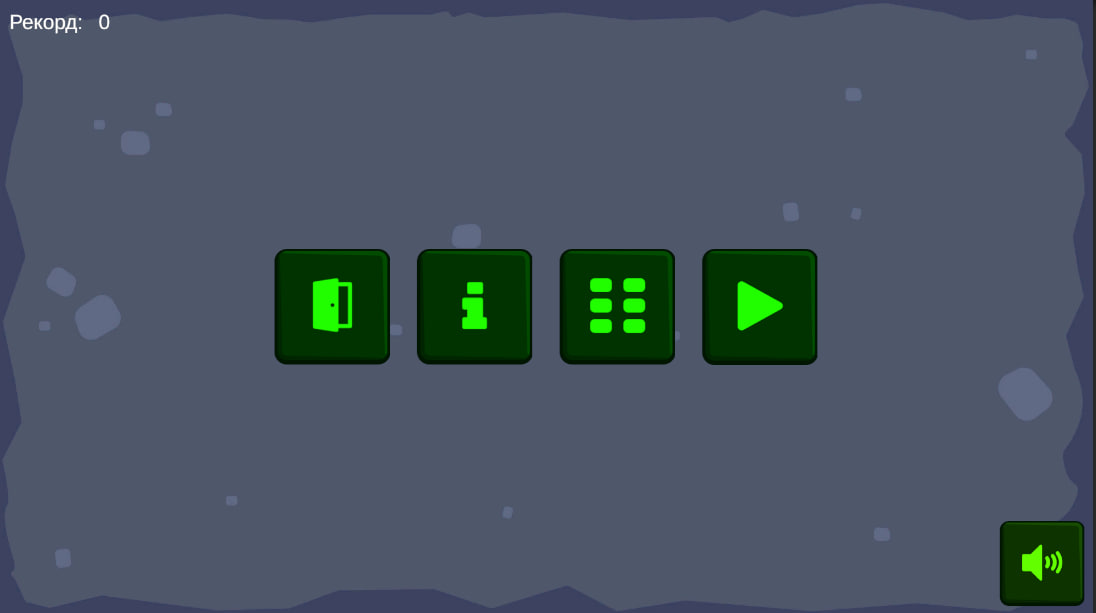
\includegraphics[width=0.8\linewidth]{images/menu.jpg}
\caption{Главное меню игры}
\label{fig:mpr}
\end{figure}

Окно успешно открывается, все элементы присутствуют.При нажатии на кнопку «Играть», происходит переход в игровую сцену в обычный режим игры(режим без препятсвии).

\begin{figure}[h]
\centering
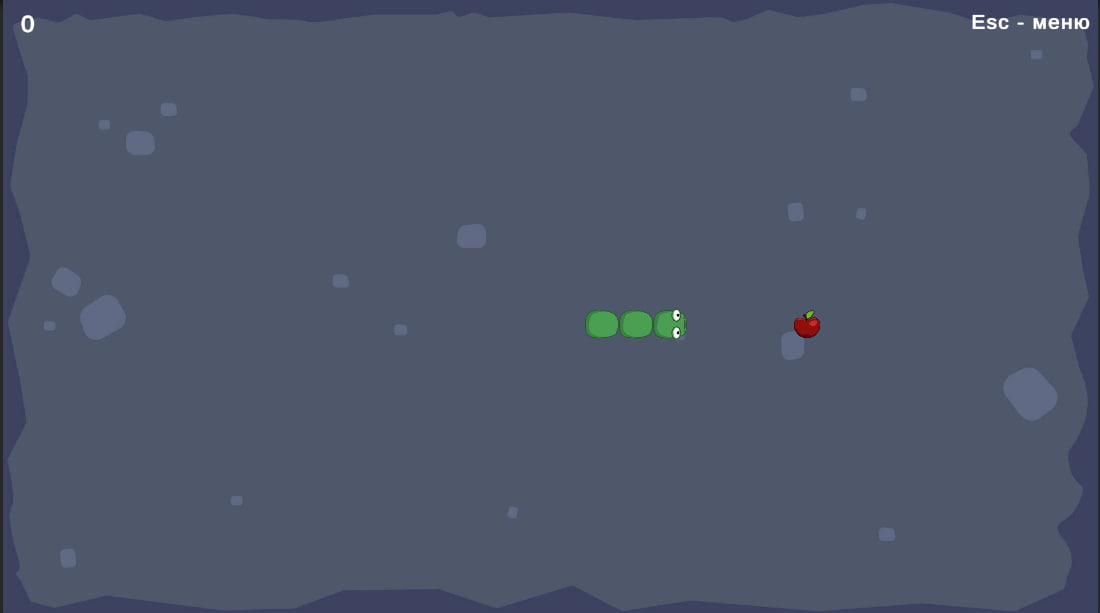
\includegraphics[width=0.8\linewidth]{images/basegame.jpg}
\caption{Режим "Обычный"}
\label{fig:mpr}
\end{figure}

После того как змейка съела яблоко, спавниться бомба с таймером, равным длине змейки.

\begin{figure}[h]
\centering
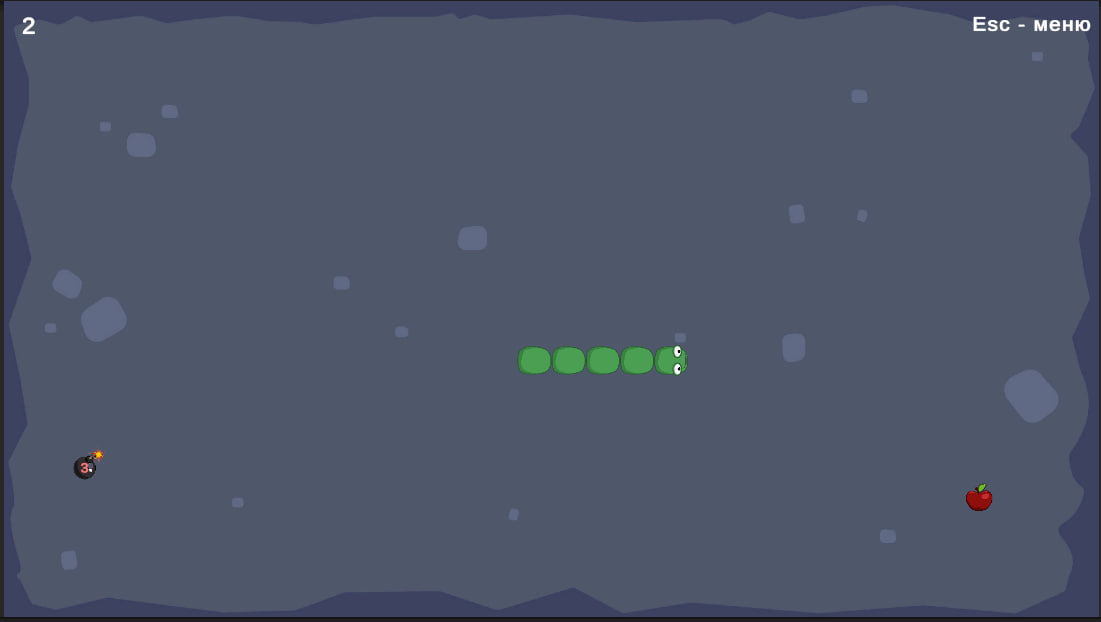
\includegraphics[width=0.8\linewidth]{images/bomb.jpg}
\caption{Спавн "Бомбы"}
\label{fig:mpr}
\end{figure}

Режим "Обычный" успешно работает, все механики реализованы. Далее проверяем режим игры со случайными препятствиями.  Для этого необходимо перейти с главного меню в "Уровни", где можно выбрать данный режим, а также можно запустить редактор карт.

\begin{figure}[h]
\centering
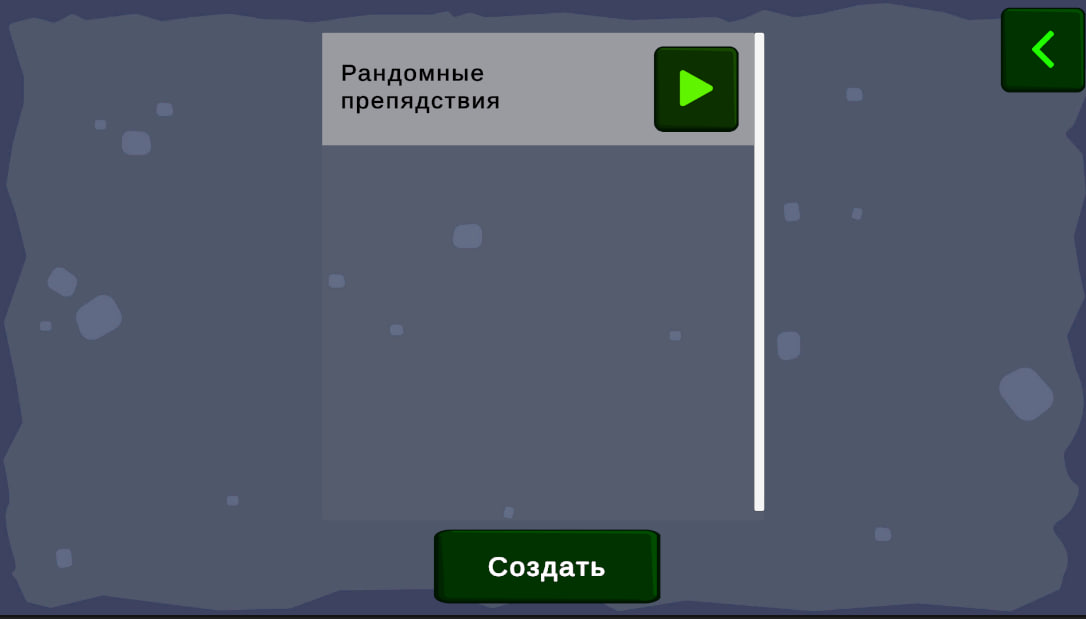
\includegraphics[width=0.8\linewidth]{images/urovni.jpg}
\caption{Режим со случайными препятствиями и редактор карт}
\label{fig:mpr}
\end{figure}

Кнопка "Уровни" успешно работает. Проверяем реализацию случайных препятствии.

\begin{figure}[h]
\centering
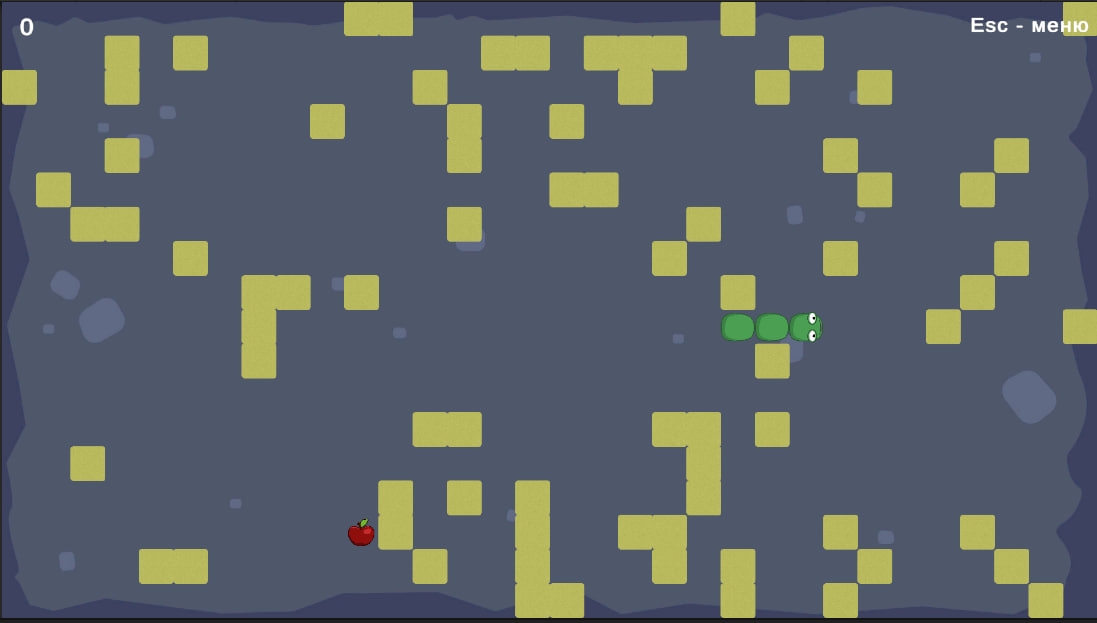
\includegraphics[width=0.8\linewidth]{images/random.jpg}
\caption{Режим игры со случайными препятсвиями}
\label{fig:mpr}
\end{figure}

Режим игры со случайными препятствиями успешно работает.
Необходимо проверить работоспособность редактора карт. Для создания карты, нужно нажать кнопку "Создать" и далее появляется пустое поле, где можно раставлять препятствия

\begin{figure}[h]
\centering
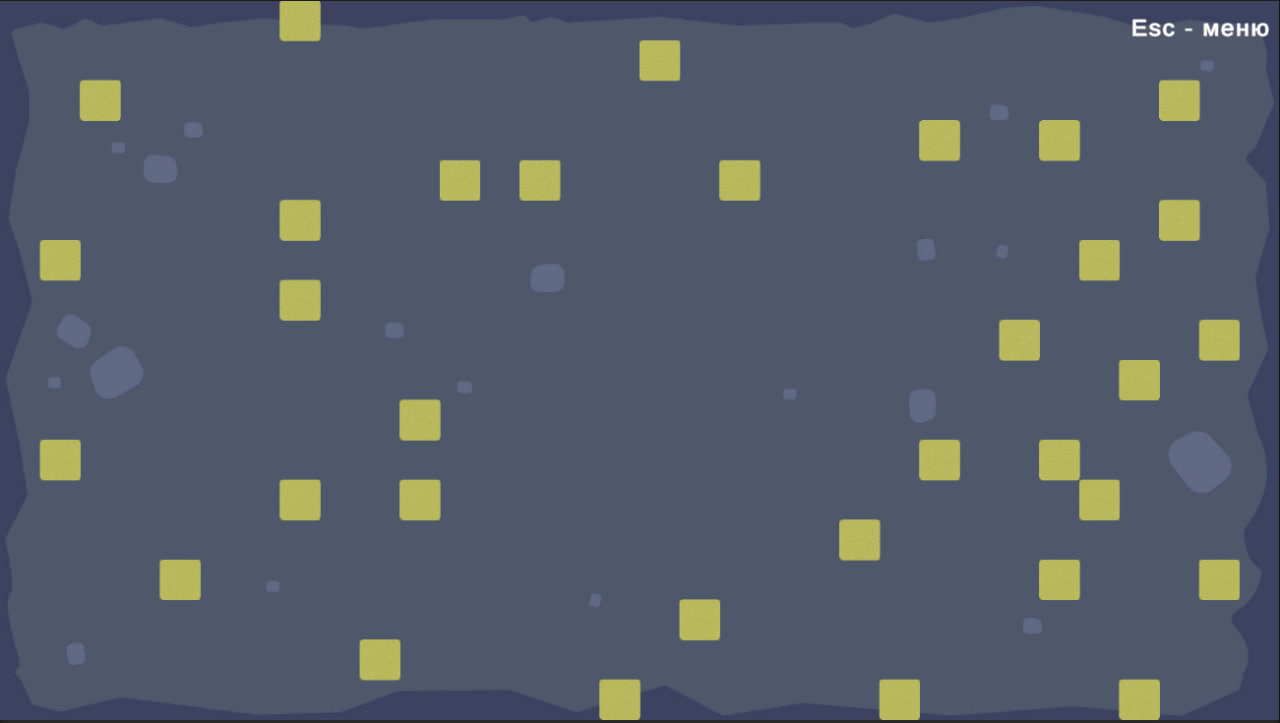
\includegraphics[width=0.8\linewidth]{images/editor.jpg}
\caption{Редактор карт}
\label{fig:mpr}
\end{figure}

\begin{figure}[h]
\centering
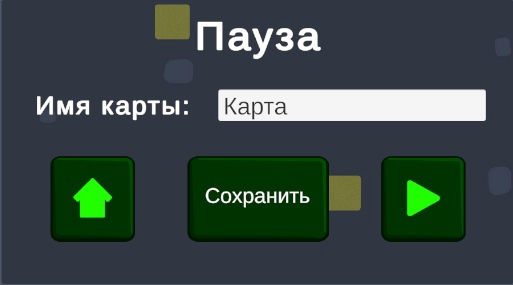
\includegraphics[width=0.8\linewidth]{images/UChfYsjxFxY.jpg}
\caption{Сохранение карты}
\label{fig:mpr}
\end{figure}

\begin{figure}[h]
\centering
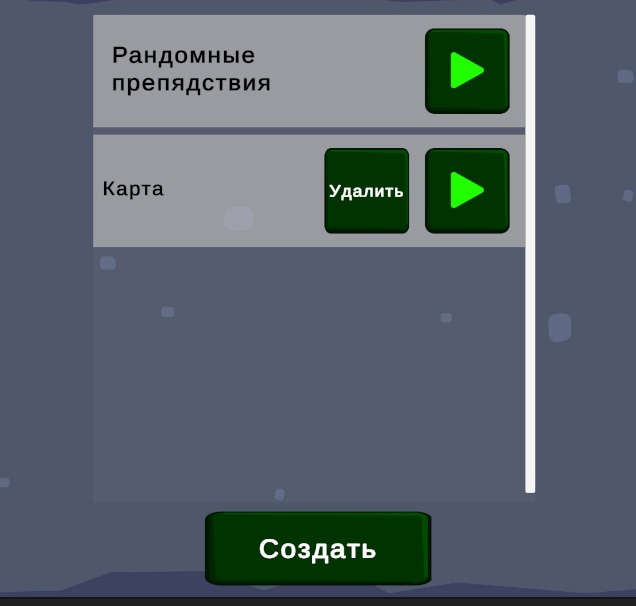
\includegraphics[width=0.8\linewidth]{images/bbva5UFq2a4.jpg}
\caption{Появление созданной карты в меню "Уровни"}
\label{fig:mpr}
\end{figure}

Редактор карт и все необходимые механики для нее были реализованы успешно.


% Подключение третий главы (практическая часть с тестированием:
\include{chapter-3-report-csae.tex}

\chapter*{Заключение}

В ходе данной курсовой работы была исследована и реализована разработка игры "Змейка" на платформе Unity. В процессе создания игры были изучены основные принципы разработки игрового проекта, такие как управление персонажем, обработка столкновений, генерация объектов на сцене и управление сценами.

Основная цель проекта заключалась в создании игры, которая была бы интересной для игроков и демонстрировала базовые навыки разработки игр на Unity. Реализация игры "Змейка" включала в себя создание игрового процесса, визуального дизайна, взаимодействия пользовательского ввода и обработки игровой логики.

Разработка игры "Змейка" на Unity позволила закрепить знания по созданию игровых проектов, использованию различных компонентов движка Unity, а также работе с кодом на языке программирования C\#.

В процессе реализации были преодолены трудности и проблемы, что позволило улучшить навыки проектирования игровых механик и обучило решению возникающих задач в процессе разработки.

Таким образом, создание игры "Змейка" на платформе Unity позволило погрузиться в процесс разработки игрового проекта, усовершенствовать навыки программирования и дизайна игр, а также приобрести опыт работы с игровым движком Unity.

\end{document}

